\documentclass[10pt,conference,compsocconf]{IEEEtran}

\usepackage{hyperref}
\usepackage{graphicx}	% For figure environment

\begin{document}
	\title{Project 1 - finding the Higgs Boson}
	
	\author{
		L\'ea Bommottet, Nicolas Brunner, Karine Perrard\\
		\textit{CS-433 Machine Learning, EPFL, Switzerland}
	}
	
	\maketitle
	\begin{abstract}
		Regression is an important point of machine learning, since it may predict future data. Applying regression to a known dataset and output gives a parameter that can be later applied on dataset to predict an output. There are several models that can be used to achieve regression, and some of them fit better for some data.
	\end{abstract}
	\section{Introduction}
	
	In this project we have to solve a binary classification problem. In function of a vector of features regarding a proton collision event, we have to determine if this collision produced an Higgs boson or another process,
	there are at most 30 parameters provided for each classification. We have to implement and use machine learning methods, then feature processing and engineering to solve this problem.
	
	\section{Models and methods}
	
	\subsection{Choice of Models}
	First of all, we have to select the core of our model. In this project, there is 6 possible models on which we can base.
	\subsubsection{Linear regression using gradient descent}
	
	This model try to minimize the error of the function, by moving the vector w in the reverse trajectory of the gradient.
	$$w^{(t+1)}=w^{(t)} -\gamma \nabla L(w^{(t)})$$
	$$e = y-Xw$$
	$$\nabla L(w) = -\frac{1}{N}X^te$$
	
	\subsubsection{Linear regression using stochastic gradient descent}
	
	The error function is defined as a sum over the training errors: \\
	$$ L(w) = \sum\limits_{n=1}^N L_n(w)$$
	As for gradient descent, we want to follow the gradient, but this time the updating step is done on the cost contributed by one of the training examples. We can also compute the gradient on a subset of the examples, this is mini-batch stochastic gradient descent.
	$$w^{(t+1)}=w^{(t)} -\gamma \nabla L_n(w^{(t)})$$
	
	
	\subsubsection{Least squares regression using normal equations}
	
	We try to solve: $\nabla L(w^*) = 0$
	
	Then we derive
	$$w^* = (X^\top X)^{-1}X^\top y$$
	and a unknown data-point would have 
	$$\hat y_m := x_m^\top w^*$$
	
	\subsubsection{Ridge regression using normal equations}
	
	We want to punish complex models and conversely choose simpler ones.
	In the case of ridge regression, we add a regularizer $\Omega(w) = \lambda||w||_2^2$ in the quest to minimize w:
	$$\min\limits_{w} L(w) + \Omega(w)$$
	the explicit solution of w become:
	$$w_{ridge}^* = (X^\top X+2N\lambda I)^{-1}X^\top y$$
	\subsubsection{Logistic regression using gradient descent or SGD}
	
	The problem is about separating the outputs into different labels. To do so we use the logistic function, that gives values in the range [0, 1]:
	$$\sigma(z) := \frac{e^z}{1 + e^z}$$
	Again we want to minimize the cost function defined as 
	$$ L(w) = \sum\limits_{n=1}^N ln[1 + e^{x_n^Tw}] - y_nx_n^Tw$$
	To compute the model, we use gradient descent. The formula is 
	$$w^{(t+1)}=w^{(t)} -\gamma \nabla L(w^{(t)})$$
	where  $$\nabla L(w) = X^T[\sigma(Xw) - y]$$ 
	
	\subsubsection{Regularized logistic regression using gradient descent or SGD}
	We can have troubles if the data is linearly separable. In that case, any vector \textbf{w} having the right direction is solution gives the minimum for \textbf{L(w)}. The goal of regularization is to add a penalty term, which is the length of the vector.
	$$ w* = argmin_w - \sum\limits_{n=1}^N ln p(y_n|x_n^T, w) + \frac{\lambda}{2}||w||^2 $$
	
	
	The reason we based our model on logistic regression is because we have the least global error on the dataset. Tb. ~\ref{error_table}
	
	Furthermore, in function of the feature named "fit", some parameters are unavailable. Thanks to this important information, we don't train only one model, but 4, since "fit" can be {0,1,2,3}.
	This idea reduce our global error, when compared to an single model without this separation. Fig.~\ref{fig:noSepFunction}
	
	\begin{figure}[tbp]
		\centering
		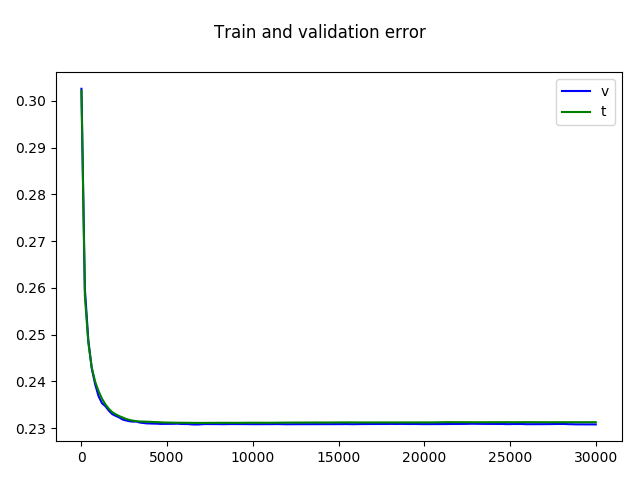
\includegraphics[width=\columnwidth]{valid_train_error_with_thresh_no_jet.png}
		\caption{Train and Validation error with no separation according to number of iterations}
		\vspace{-3mm}
		\label{fig:noSepFunction}
	\end{figure}
	
	\subsection{Choice of parameters}
	We use cross-validation by K-fold to compute the most efficient lambda and gamma; the plot are below in Fig.~\ref{fig:crossValidation}. The parameters that reduce most the train error in our function are lambda = $10^{-5}$ and gamma = $10^{-5}$.
	
	\subsection{Choice of features}
	
	We can improve our model by adding new features, which are function of other parameters. We want more features that have a Normal distribution. 
	\begin{description}
		\item[Natural logarithm] \ \\
		Applying the logarithm on a parameter can highlight its Normal behavior. One example is this function on the feature 21 (Fig.~\ref{fig:feature21function}). In this case, we notice a much nicer Gaussian distribution on the values, than the initial data. By doing an exhaustive research, we find that the useful parameters with this function are \{0, 1, 2, 3, 4, 5, 8, 9, 10, 13, 16, 19, 21, 23, 26, 29\}, when discarding the NaN value.
		\item[Square root] \ \\
		Same as the natural logarithm, the square root can bring out a normal distribution. The feature 21 is also transformed with this function in our model (Fig.~\ref{fig:feature21function}). Again if we don't consider the NaN value, the parameters \{0, 13, 16, 21, 23, 26, 29\} have a Normal behavior under the square root
		\item[Threshold] \ \\
		Some features are mostly distributed along two peaks. In that case we move values to their closest peak to get two well defined peaks. This is the case for parameters \{11, 12\}.
		\item[Nothing max] \ \\
		Some features have no defined distribution, but their values explode to big numbers. In that case we divide by maximum to get new value in range [0, 1]. Such distributed parameters are parameters \{6, 14, 17, 24, 27\}
		\item[Nothing norm] \ \\
		Some features have no distribution and their values are already between 0 and 1. For parameter 7 we do nothing.
		\item[Distance] \ \\
		When we plot 2 parameters in a graph, we can find some correlation between (Fig.~\ref{fig:feature1825}). To reduces this property to a normal distribution, we compute the Manhattan distance, to flatten all the perpendicular result on the plot $y = -x$. The Manhattan distance is computed as follow:
		$$dist(x_1, x_2) = |x_1 - x_2|$$ 
		
		\item[$N^{th}$ power] \ \\
		Some feature sometimes have a better behavior when they are raised to a power greater than 2, as it is the case for feature 19 when raise to the cube (Fig.~\ref{fig:feature19})
	\end{description}
	
	\section{Results}
	\begin{figure}[tbp]
		\centering
		\includegraphics[width=\columnwidth]{21_0_modified}
		\caption{Function applied on the data of the feature 21}
		\vspace{-3mm}
		\label{fig:feature21function}
	\end{figure}
	\begin{figure}[tbp]
		\centering
		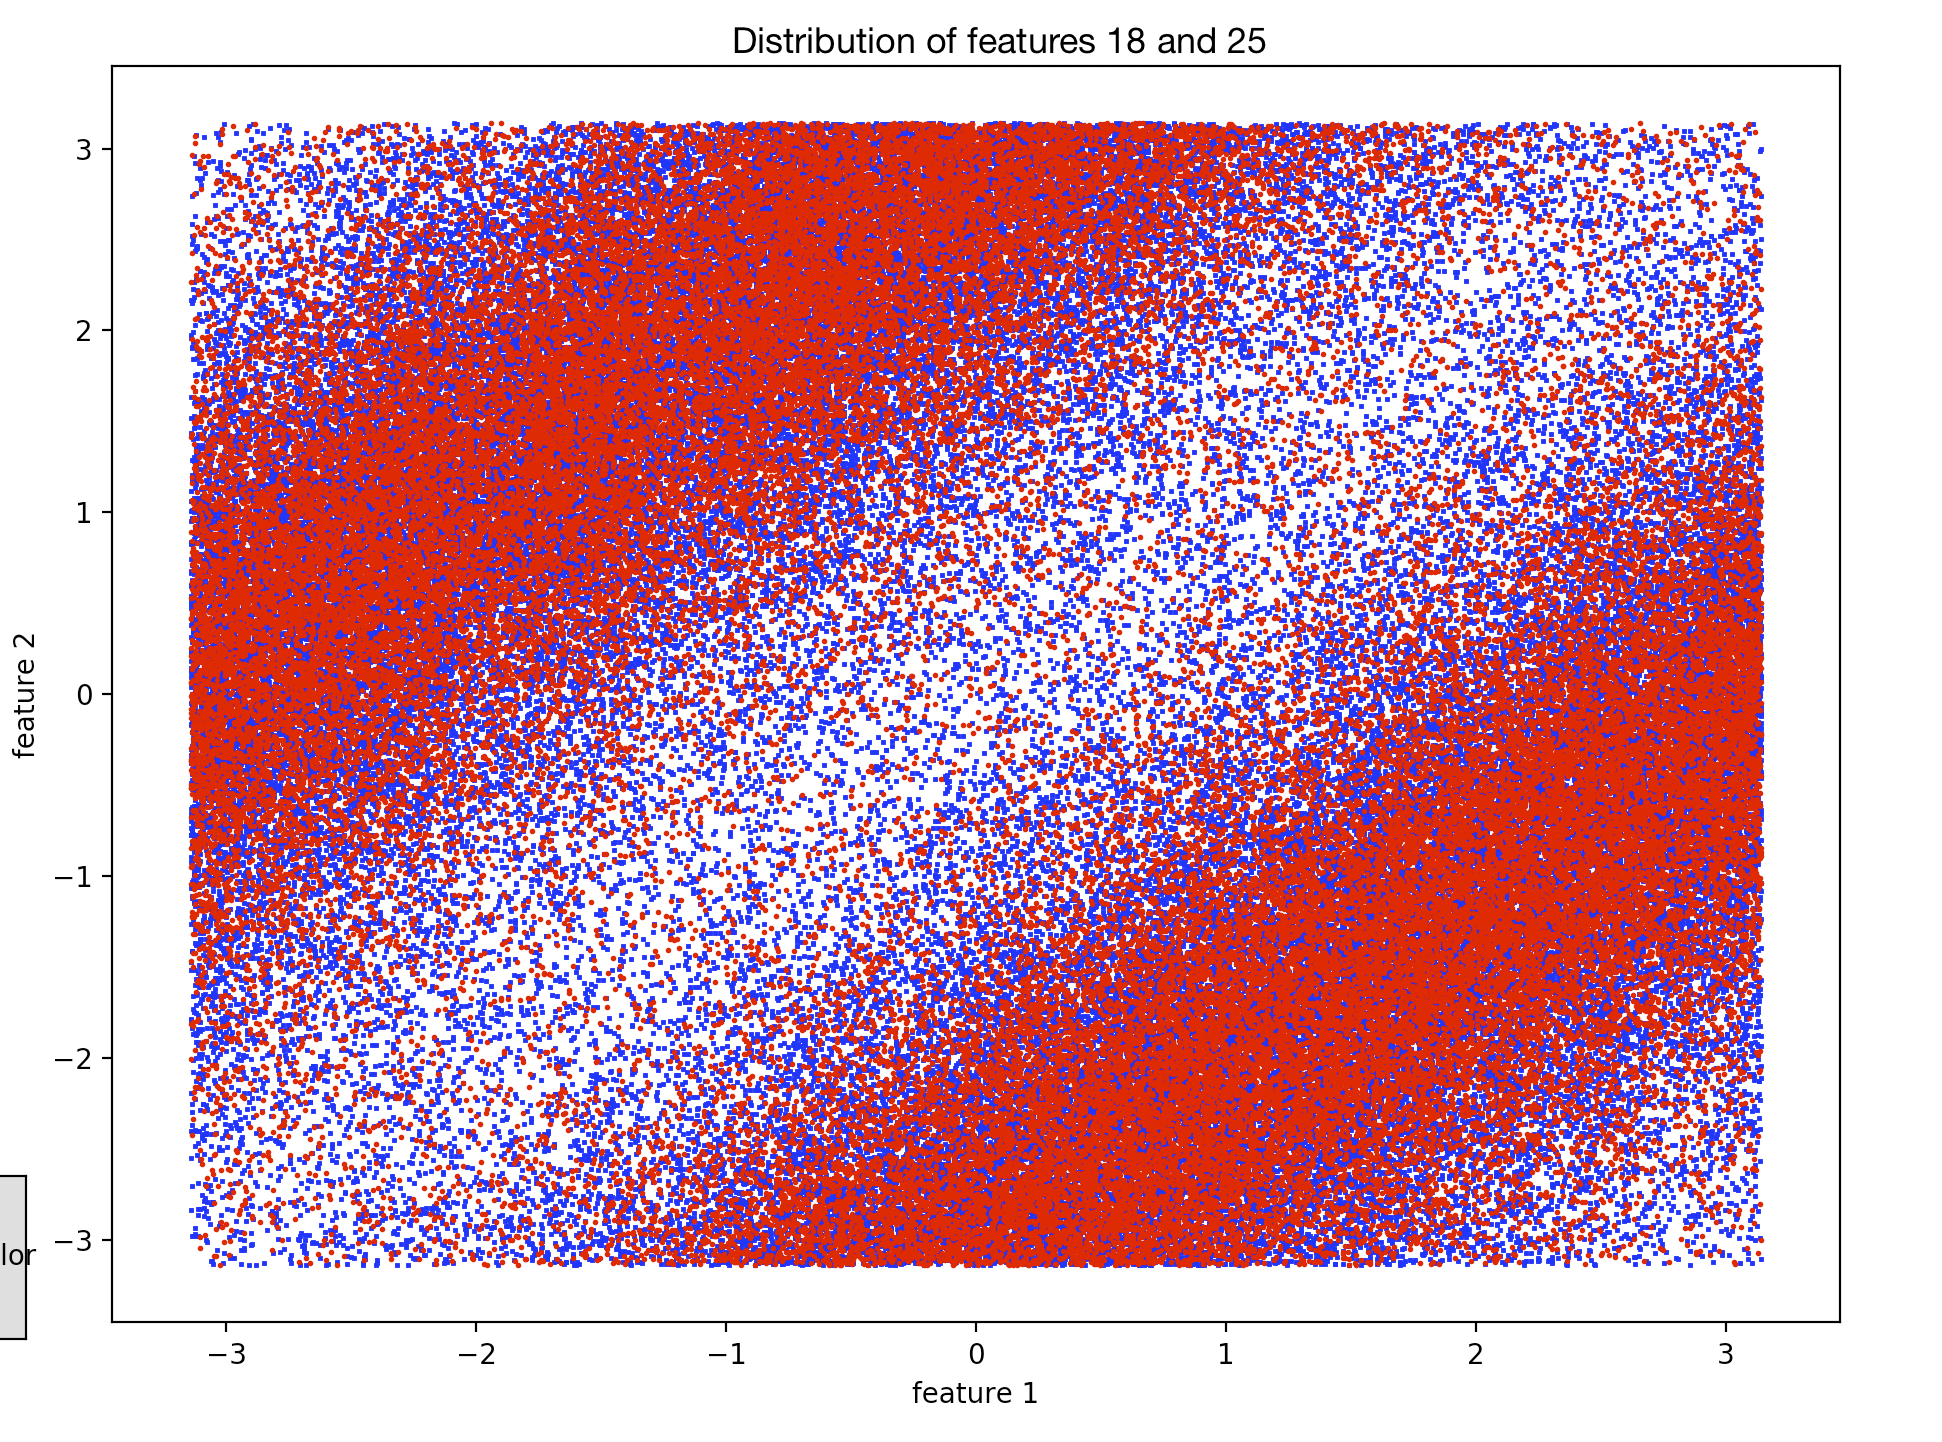
\includegraphics[width=\columnwidth]{features18_25}
		\caption{Repartition of features 18 ans 25}
		\vspace{-3mm}
		\label{fig:feature1825}
	\end{figure}
	\begin{figure}[tbp]
		\centering
		\includegraphics[width=\columnwidth]{CrossValidation}
		\caption{Cross validation for lambda and gamma}
		\vspace{-3mm}
		\label{fig:crossValidation}
	\end{figure}
	\begin{figure}[tbp]
		\centering
		\includegraphics[width=\columnwidth]{19_3_modified}
		\caption{Function applied to feature 19}
		\vspace{-3mm}
		\label{fig:feature19}
	\end{figure}
	As we can see in table ~\ref{error_table}, the best prediction possible 
	\begin{table}[]
		\centering
		\caption{Global error percentage for each model and method}
		\label{error_table}
		\begin{tabular}{|l|llllll|}
			\hline
			Model & \begin{tabular}[c]{@{}l@{}}Linear regression\\ using gradient\\ descent\end{tabular} & \begin{tabular}[c]{@{}l@{}}Linear regression\\ using stochastic\\ gradient descent\end{tabular} & \begin{tabular}[c]{@{}l@{}}Least squares\\ regression using\\ normal equations\end{tabular} & \begin{tabular}[c]{@{}l@{}}Ridge regression\\ using normal \\equations\end{tabular} & \begin{tabular}[c]{@{}l@{}}Logistic regression\\ using gradient\\ descent or SGD\end{tabular} & \begin{tabular}[c]{@{}l@{}}Regularized logistic\\ regression using\\ gradient descent \\or SGD\end{tabular} \\ \hline
			\begin{tabular}[c]{@{}l@{}}1 jet\\ (3000 iterations)\end{tabular} & 1.0 & 0.36664 & 0.26512 & 0.265312 & 0.3196 & 0.319616 \\ \hline
			\begin{tabular}[c]{@{}l@{}}1 jet with feature processing\\ (3000 iteration)\end{tabular} & 0.325024 & 0.338288 & 0.240192 & 0.256256 & 0.22632 & 0.226352 \\ \hline
			\begin{tabular}[c]{@{}l@{}}4 jets\\ (3000 iterations)\end{tabular} & 1.0 & 0.898050 & 0.248029 & 0.250557 & 0.383947 & 0.431784 \\ \hline
			\begin{tabular}[c]{@{}l@{}}4 jets with feature processing\\ (3000 iterations)\end{tabular} & 0.302155 & 0.338330 & 0.224749 & 0.239293 & 0.195069 & 0.195053 \\ \hline
			\begin{tabular}[c]{@{}l@{}}4 jets with feature processing\\ (30000 iterations)\end{tabular} & 0.255292 & 0.282860 & 0.224748 & 0.239292 & 0.189837 & 0.189933 \\ \hline
		\end{tabular}
	\end{table}
	Separating our model into 4 different ones was a great idea, reducing considerably our global error (Fig.~\ref{error_table}) as well as including more preprocessed features. Those added criterion improve the quality of our model, adjusting from ??? to ???.    
	0.18\% of error is kinda ok with the simplicity of the core models. If we want to improve it more, we would need to find more useful parameters to boost our data.
	
	\section{Summary}
	The best prediction we could get to was obtained by using logistic regression on processed input data.
	
	\begin{thebibliography}{1}
		
		\bibitem{notes} John W. Dower {\em Readings compiled for History
			21.479.}  1991.
		
		\bibitem{impj}  The Japan Reader {\em Imperial Japan 1800-1945} 1973:
		Random House, N.Y.
		
		\bibitem{norman} E. H. Norman {\em Japan's emergence as a modern
			state} 1940: International Secretariat, Institute of Pacific
		Relations.
		
		\bibitem{fo} Bob Tadashi Wakabayashi {\em Anti-Foreignism and Western
			Learning in Early-Modern Japan} 1986: Harvard University Press.
		
	\end{thebibliography}
	
\end{document}
